\documentclass{article}

\usepackage{tcolorbox}
\usepackage[nonatbib, final]{nips}

\makeatletter
\renewcommand{\@noticestring}{
  \begin{center}
    Progress Report. Work in Progress.
  \end{center}
}
\makeatother

\usepackage[T1]{fontenc}
\usepackage[utf8]{inputenc}

\usepackage{microtype}

\usepackage[numbers]{natbib} % Natbib Citations
\usepackage{soul} % Underline, Strikethrough
\usepackage{afterpage} % Blank Page
\usepackage[super]{nth} % 1st, 2nd, etc.
\makeatletter
\@ifclassloaded{beamer}{}{
  \usepackage[shortlabels, inline]{enumitem}
} % Inline Enumeration
\makeatother
% Tables and Figures
\usepackage{float, graphicx, wrapfig, subcaption}
\usepackage[export]{adjustbox} % Vertical Alignment
\usepackage{booktabs, tabularx, multirow, tablefootnote}
% Monospaced Code Blocks
\usepackage{fancyvrb, listings}
% Math Packages
\usepackage{nicefrac}
\usepackage{amsmath, amsfonts}

\lstset{ %
  backgroundcolor=\color{white},   % choose the background color; you must add \usepackage{color} or \usepackage{xcolor}; should come as last argument
  basicstyle=\bfseries\ttfamily,   % the size of the fonts that are used for the code
  breakatwhitespace=false,         % sets if automatic breaks should only happen at whitespace
  breaklines=true,                 % sets automatic line breaking
  captionpos=b,                    % sets the caption-position to bottom
  commentstyle=\color{gray},       % comment style
  deletekeywords={...},            % if you want to delete keywords from the given language
  escapeinside={\%*}{*)},          % if you want to add LaTeX within your code
  extendedchars=true,              % lets you use non-ASCII characters; for 8-bits encodings only, does not work with UTF-8
  % frame=single,                    % adds a frame around the code
  keepspaces=true,                 % keeps spaces in text, useful for keeping indentation of code (possibly needs columns=flexible)
  keywordstyle=\color{blue},       % keyword style
  language=C++,                    % the language of the code
  % morekeywords={*,...},            % if you want to add more keywords to the set
  numbers=none,                    % where to put the line-numbers; possible values are (none, left, right)
  numbersep=5pt,                   % how far the line-numbers are from the code
  numberstyle=\color{black},       % the style that is used for the line-numbers
  rulecolor=\color{black},         % if not set, the frame-color may be changed on line-breaks within not-black text (e.g. comments (green here))
  showspaces=false,                % show spaces everywhere adding particular underscores; it overrides 'showstringspaces'
  showstringspaces=false,          % underline spaces within strings only
  showtabs=false,                  % show tabs within strings adding particular underscores
  stepnumber=1,                    % the step between two line-numbers. If it's 1, each line will be numbered
  stringstyle=\color{red},         % string literal style
  tabsize=4,                       % sets default tabsize to 4 spaces
  % title=\lstname                   % show the filename of files included with \lstinputlisting; also try caption instead of title
}

\newcommand{\Emph}[1]{\ul{\textbf{#1}}}

\makeatletter
\@ifpackageloaded{hyperref}{}{\usepackage{hyperref}}

\g@addto@macro{\UrlBreaks}{\UrlOrds}
\g@addto@macro{\UrlBreaks}{\do\/%
\do\a\do\b\do\c\do\d\do\e\do\f\do\g\do\h\do\i\do\j\do\k\do\l\do\m\do\n\do\o\do\p\do\q\do\r\do\s\do\t\do\u\do\v\do\w\do\x\do\y\do\z%
\do\A\do\B\do\C\do\D\do\E\do\F\do\G\do\H\do\I\do\J\do\K\do\L\do\M\do\N\do\O\do\P\do\Q\do\R\do\S\do\T\do\U\do\V\do\W\do\X\do\Y\do\Z%
\do\1\do\2\do\3\do\4\do\5\do\6\do\7\do\8\do\9\do\0\do\.}
\makeatother


\title{EmRNN: Memory Footprint Reduction for Neural Machine Translation}

\author{
  Bojian Zheng \\
  EcoSystem Research Group, Department of Computer Science \\
  University of Toronto \\
  \texttt{bojian@cs.toronto.edu} \\
}

\begin{document}

\maketitle

\section{GroundHog Model}

\subsection{Dataset}

The training dataset was selected to be the IWSLT15 English-Vietnamese dataset, 
which was obtained from the \Emph{Tensorflow NMT} \cite{tf-nmt} repository.

\subsection{Model Description}

\begin{figure}[ht]
  \begin{center}
    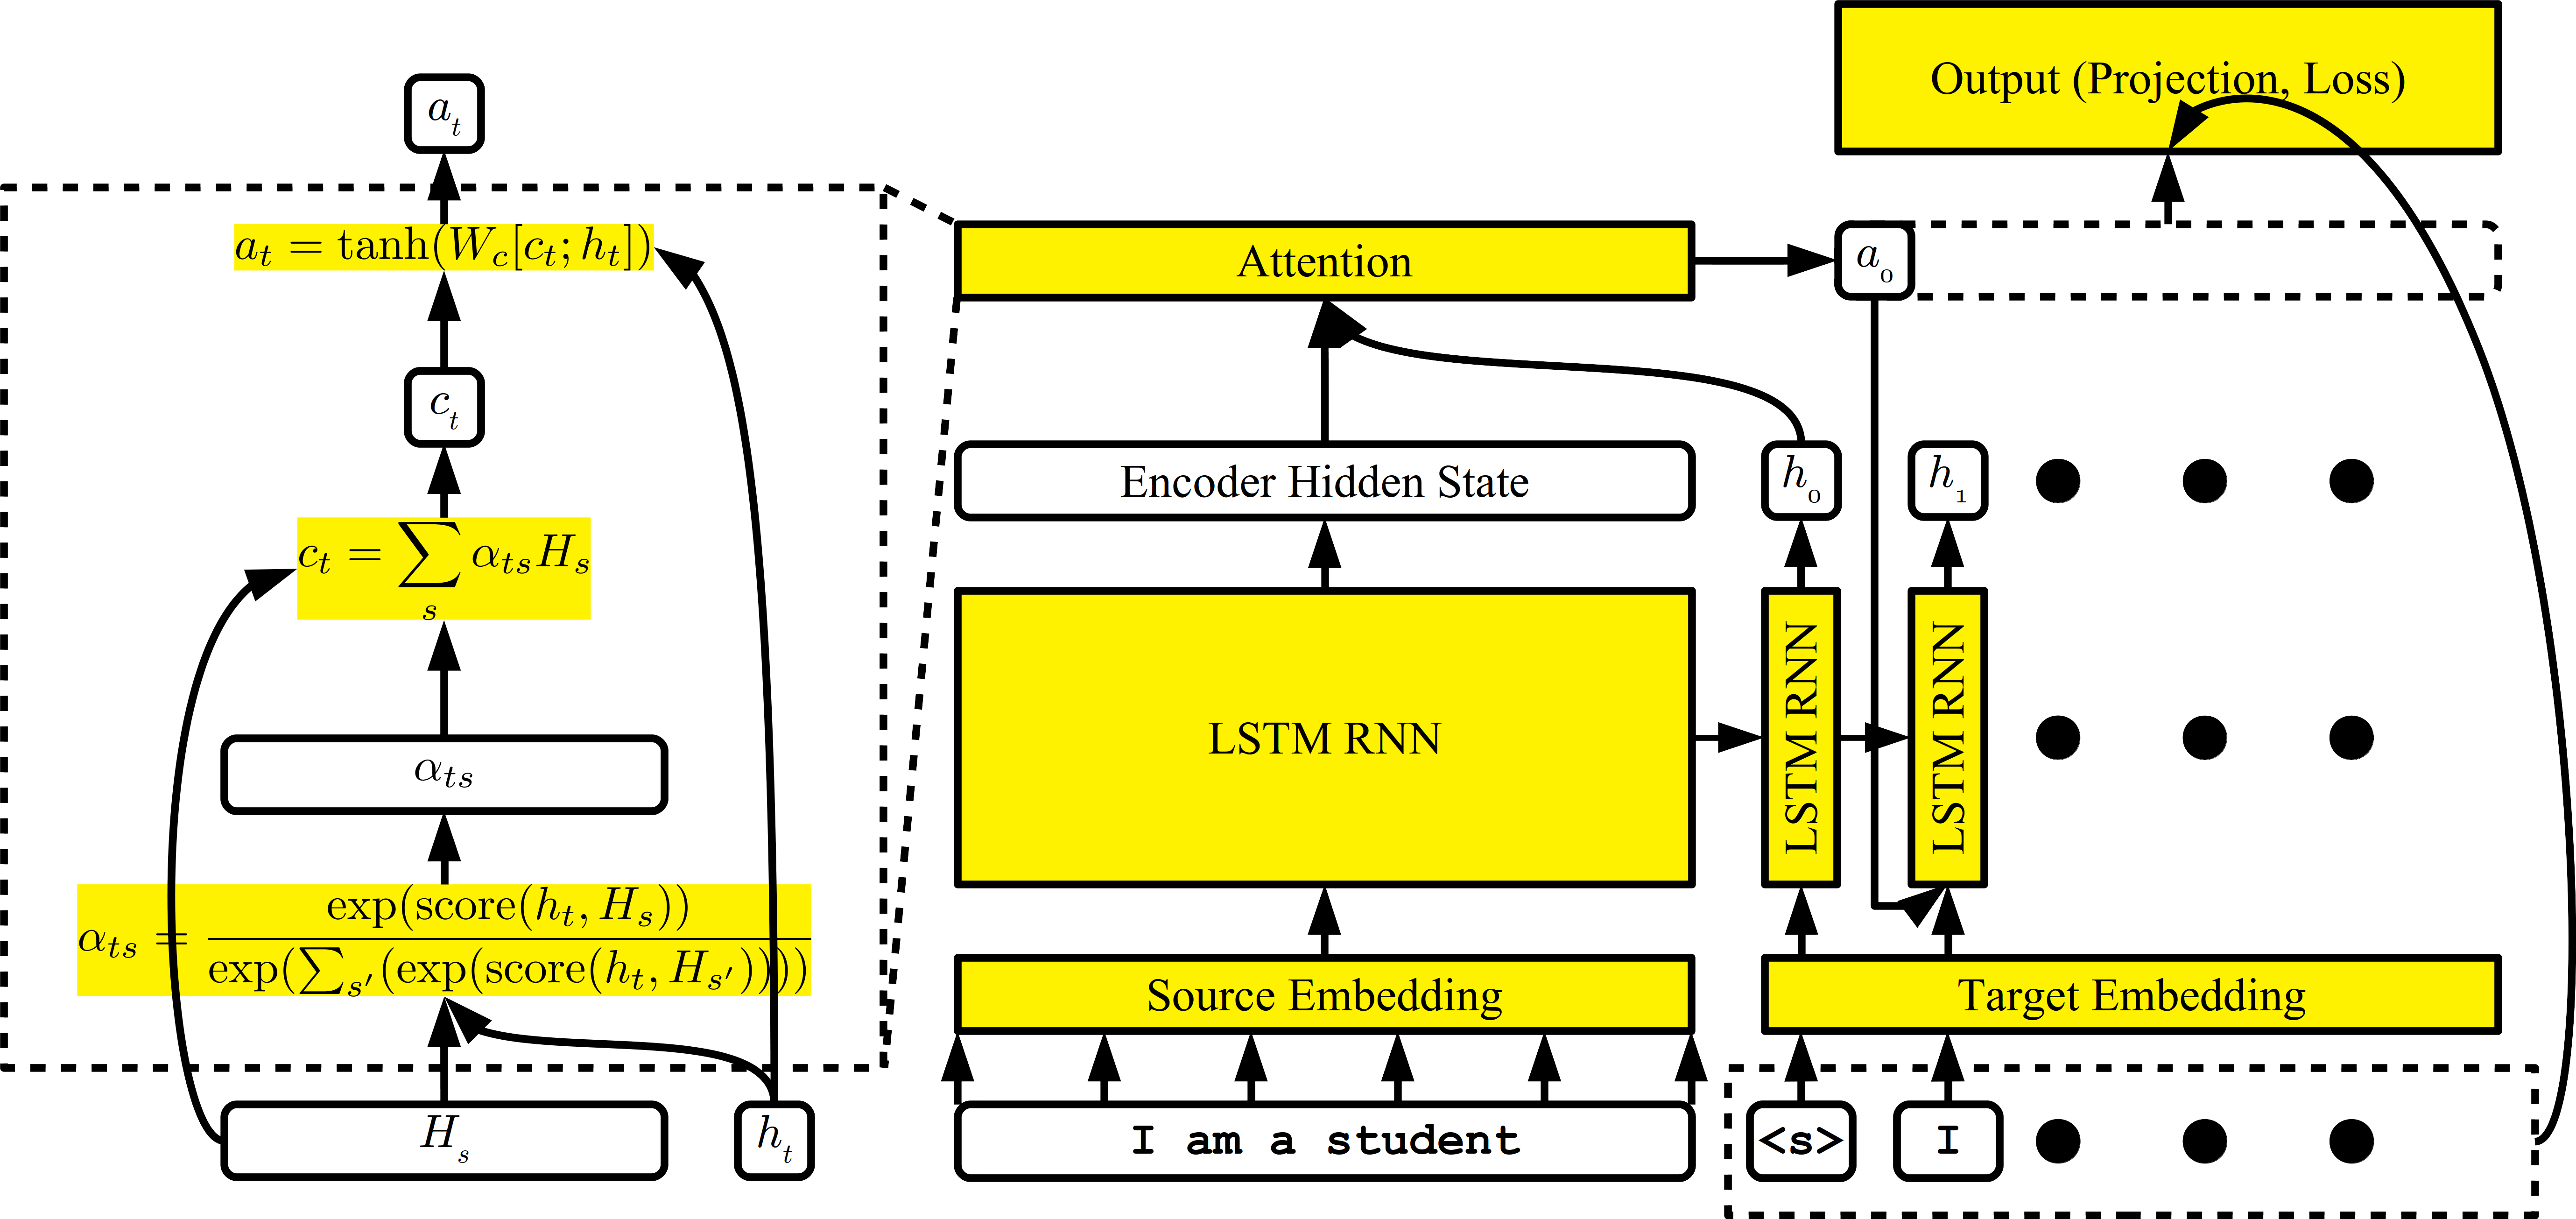
\includegraphics[width=0.99\linewidth]{./graphs/groundhog.png}
    \caption{Visualization of the Sockeye Groundhog model. 
    Rounded boxes denote placeholders or intermediate variables and yellow rectangles denote computation layers.}
  \end{center}
\end{figure}

All frameworks used \(B=80\), \(\max{|S|}=\max{|T|}=50\).

\paragraph{Embedding}
The embedding layers for the encoder and decoder were chosen to have \(H=500\).
There is no sharing between the encoder and decoder embedding weights.

\paragraph{Encoder}
1-layer bidirectional LSTM.

\paragraph{Decoder}
1-layer unidirectional LSTM with MLP attention with \(H=512\).

\begin{tcolorbox}
  The formula for MLP (a.k.a. Bahdanau's) attention is given by 
  \[\text{score}(h_t, H_s)=V_\text{h2s}\tanh(W_\text{q2h}h_t+W_\text{e2h}H_s)\]
  where \(\text{q, e, h}\) stand respectively for query (\(h_t\)), encoder (\(H_s\)), and hidden.
\end{tcolorbox}

Both RNNs have been chosen to have \(H=1000\), and input dropout probability \(p=0.3\).

\paragraph{Optimizer}
The optimizer is the Adam optimizer with gradient clipping \(1.0\).

\subsection{Methodology}

The way we are going to profile the memory goes as follows:
\begin{enumerate*}[(1)]
  \item obtain the memory usage report from \lstinline{nvprof}
  \label{nvprof}
  \item add a accumulator before the \lstinline{cudaMalloc} function call and 
  see whether it matches with the result obtained in \ref{nvprof}
  \label{cudaMalloc}
  \item compute the theoretical allocation and 
  see whether it matches with the result obtained in \ref{cudaMalloc}
\end{enumerate*}.

\subsection{Results}

\paragraph{Acknowledgement}
The memory profiling result is obtained from the MXNet memory profiling tool developed by \Emph{Abhishek Tawari}.

On the groundhog model, Sockeye \cite{sockeye} was able to obtain \(20.7\) BLEU score on the validation dataset,
which is lower than what has been reported in the 
\Emph{Tensorflow NMT} \cite{tf-nmt} repository (\(\sim\) \(23\) BLEU score).
However, due to the fact that the groundhog model is 
the simplest model. We do argue that Sockeye has been training properly.

The total consumed memory is \(4.4\) GB, and the breakdown goes as follows:

\paragraph{!Important}
Please carefully note the followings:
\begin{enumerate*}[(1)]
  \item For all the variables below, unless otherwise specified, will have \Emph{a base multiplier of} \(4\times\),
  which is the size of single-precision floating point value.
  \item For all the \Emph{weights} below, unless otherwise specified, will have \Emph{an additional multiplier of} \(2\times\),
  which is because weights need to allocate extra spaces for gradients.
  \item \Emph{NOT all memory consumptions are reported}. 
  The following computation does not take into account memory consumptions that are 
  relatively insignificant or caused by library (e.g. cuDNN) overhead.
  \item The profiling does NOT take \Emph{"dynamic"} memory allocation into account. 
  By "dynamic" we mean the behavior of transferring storage temporarily from GPU or CPU,
  or freeing the temporary workspace.
\end{enumerate*}

\newcommand{\MB}{\text{ }\mathtt{MB}}

\paragraph{Embedding}
\begin{itemize}
  \item \lstinline{Source} Weights: \(|V_\text{src}|\times H\Rightarrow  7710\times 500\times 4\times 2=31\MB\)
  \item \lstinline{Target} Weights: \(|V_\text{tgt}|\times H\Rightarrow 17192\times 500\times 4\times 2=69\MB\)
\end{itemize}

\paragraph{Encoder}
\begin{itemize}
  \item \lstinline{ Forward i2h} Weight: \((4\times \frac{1}{2}H_\text{RNN})\times \frac{1}{2}H_\text{RNN}\Rightarrow 
  4\times 1000\times 1000\times 4\times 2=8\MB\)
  \footnote{The reason why it is \(\frac{H}{2}\) is because in the Sockeye implementation of \lstinline{BidirectionalRNNEncoder},
  the real hidden dimension is half of the given one. 
  This can be verified \href{https://github.com/awslabs/sockeye/blob/3280f7b0111b705d2218096121a20f6471f1f4e8/sockeye/encoder.py\#L874}{here}.}
  \item \lstinline{ Forward h2h} Weight: \((4\times \frac{1}{2}H_\text{RNN})\times \frac{1}{2}H_\text{RNN}\Rightarrow 
  4\times 1000\times 1000\times 4\times 2=8\MB\)
  \item \lstinline{Backward h2h} Weight: \((4\times \frac{1}{2}H_\text{RNN})\times \frac{1}{2}H_\text{RNN}\Rightarrow 
  4\times 1000\times 1000\times 4\times 2=8\MB\)
  \item \lstinline{Backward h2h} Weight: \((4\times \frac{1}{2}H_\text{RNN})\times \frac{1}{2}H_\text{RNN}\Rightarrow 
  4\times 1000\times 1000\times 4\times 2=8\MB\)
  % \item Feature Map: \(2\times T\times \text{FeatureMap}_\text{cell}\),
  % where \(2\times\) is because the encoder is bidirectional,
  % \(T\) is the maximum of time steps unrolled, and
  % \(\text{FeatureMap}_\text{cell}\) is the feature map needed for each RNN cell,
  % which, in this case, is given by \(17\times B\times \frac{1}{2}H_\text{RNN}\).
  % The \(17\) portions consist of:
  % \begin{enumerate*}[(1)]
  %   \item \lstinline{i2h}: \(4\times\)
  %   \item \lstinline{h2h}: \(4\times\)
  %   \item \lstinline{i, f, c, (o)}: \(4\times\)
  %   \footnote{\lstinline{i, f, c, (o)} are the \(3\) (\(4\)) gates in LSTM cell, 
  %   correspond respectively to input, forget, activation, output.}
  %   \item \lstinline{slice}: \(3\times\)
  %   \item \lstinline{mul}: \(2\times\)
  %   \item \lstinline{output}: \(1\times\)
  % \end{enumerate*}.
  \item Feature Map: \(T\times \text{FeatureMap}_\text{cell}\) 
  where \(T\) is the number of unrolled time steps,
  and \(\text{FeatureMap}_\text{cell}\) is the feature map needed by each RNN cell,
  which is given by:
  \begin{enumerate*}[(1)]
    \item \lstinline{Forward}: 
  \end{enumerate*}
\end{itemize}

\paragraph{Decoder (RNN)}
\begin{itemize}
  \item \lstinline{i2h} Weight: \(4H_\text{RNN}\times (H_\text{RNN} + H_\text{tgt})\Rightarrow 
  4\times 1000\times (1000 + 500)\times 4\times 2=48\MB\)
  \item \lstinline{h2h} Weight: \(4H_\text{RNN}\times H_\text{RNN}\Rightarrow 
  4\times 1000\times 1000\times 4\times 2=32\MB\)
\end{itemize}

\paragraph{Decoder (Attention)}
\begin{itemize}
  \item \lstinline{e2h} Weight: \(H_\text{RNN}\times H_\text{Att}\Rightarrow 1000\times 512\times 4\times 2 = 4\MB\)
  \item \lstinline{q2h} Weight: \((H_\text{RNN} + H_\text{tgt})\times H_\text{Att}\Rightarrow 
  (1000 + 500)\times 512\times 4\times 2 = 6\MB\)
  \footnote{The reason why it is \((H_\text{RNN} + H_\text{tgt})\) is because the \lstinline{q2h}
  has also been taking the embedding value of previously predicated word as input 
  (this corresponds to the hyperparameter setting \lstinline{--rnn-attention-use-prev-word}).}
  \item Hidden Weight: \(H_\text{RNN}\times 2H_\text{RNN}\Rightarrow 
  1000\times 2000\times 4\times 2=16\MB\)
\end{itemize}

\paragraph{Output (a.k.a. Projection, Loss))}
\begin{itemize}
  \item \lstinline{cls} Weight: \(|V_\text{tgt}|\times H_\text{RNN}\Rightarrow 
  17192\times 1000\times 4\times 2=138\MB\)
\end{itemize}

\bibliographystyle{ACM-Reference-Format}
{\footnotesize \bibliography{bibliography}}

\end{document}
